%!TEX root = main.tex

\section{Introduction}
We will be discussing the phenomena of gravitational lensing from the point of view of general relativity. We begin by briefly reviewing the generalization of Fermat's principle to Lorentzian spacetimes. This generalization leads us to the observation that for static spacetimes there exists a one to one correspondence between null geodesics on the spacetime and geodesics of a classical Riemannian manifold (called the Fermat, or optical manifold). This allows us to bring to bear the tools of classical surface analysis and turns the study of light rays on spacetime into a classical differential geometry problem. As a specific example, we will study in detail the optical geometry of Schwarzschild. Specifically, we will show that it is necessary for a manifold to exhibit topologically nontrivial properties in order for a gravitational len to form multiple images.

% This is the subject of \textbf{optical geometry}.
% We will begin by discussing the generalisation of Fermats principle to spacetime. In order to do concrete (optical geometric) calculations, we will specialize to \textbf{static spacetimes}, which turn out to have Riemannian structure.
% In this framework, we will see that gravitational lensing is a global effect, where the topology will determine whether we can have multiple images, what the deflection angles are, etc... This will utilize the so called Gauss Bonnet theorem.

\section{Fermat's principle and optical geometry}
Herod (10-75CE) was the first to propose a variational perspective in understanding the propagation of light: he postulated that light takes the shortest path between two points.
This turns out the be correct, however, only for homogeneous media.
Fermat's principle is the sought after generalization: light always takes the shortest path in time.
We may formulate this as a calculus of variations problem in $\reals^3$ as follows.
Let $\gamma: (0,1) \to \reals^3$.
Then the curve $\gamma$ which minimizes the action $S[\gamma] \defn \int_{\gamma} \, dt = \frac{1}{c}\int_{\gamma} n \, dl$, where $n$ is a spatially varying refractive index, and $l$ is the arclength of the curve, is the physical path taken.
\begin{remark}[]\label{}
Light travels along null geodesics in spacetime, and thus the length is $0$! This means that we have to come up with a new way to formulate Fermat's principle in spacetime.
\end{remark}
%
% Recall the following definitions in the spacetime setting
%
% \begin{definition}[]\label{}
% Let $\gamma: I \to \man$ be a curve. Then $\gamma$ is a \textbf{null curve} if $g(\dot{\gamma}(\lambda), \dot{\gamma}(\lambda))=0$ for every $\lambda \in I$.
% \end{definition}
%
% \begin{definition}[]\label{}
% Let $\gamma: I \to \man$ be a curve. Then $\gamma$ is a \textbf{null geodesic} if it is a null curve, and $\nabla_{\dot{\gamma}} \dot{\gamma}$
% \end{definition}
%
% The distinction between null curves and null geodesics is of practical importance. A null geodesic satisfies the geodesic equations, implying that it is affinely parameterized. Loosely speaking, this means that the curve has constant velocity, and thus zero acceleration. This need not be the case for null curves.
%%%%%%%%%%%%%%%%%%%%%%%%%%%%%%%%%
%
%%%%%%%%%%%%%%%%%%%%%%%%%%%%%%%%%
% We introduce some notation and a result that will make our following calculations more transparent.
% \begin{definition}[]\label{}
% Let $\gamma: I \to \man$ be a curve. Then the \textbf{$i$'th coordinate image of $\gamma$ under $x$} is a map $\gamma^i_{(x)}: \reals \to \reals$ defined by
% \begin{equation}\label{}
% \gamma^i_{(x)}(\lambda) \defn (x \circ \gamma)^i (\lambda) = (x_i \circ \gamma) (\lambda)
% \end{equation}
% \end{definition}
%
% \begin{definition}[]\label{}
% Let $\gamma: I \to \man$ be a curve. Then the \textbf{velocity field along $\gamma$} is the map $\vg: \reals \to \tanb$ such that $\lambda \mapsto \vg_{(x)}^i (\lambda) \ddx{i} \rvert_{\gamma(\lambda)}$
% \end{definition}
%
% \begin{remark}[]\label{}
% Note that the components of the velocities are the derivatives of the curve image components.
% \end{remark}
% \begin{proposition}[]\label{}
% Let $\gamma: I \to \man$ be a curve, and $\vg$ be the velocity field along $\gamma$. Then
% \begin{equation}\label{}
% g(\vg(\lambda), \vg(\lambda)) = \vg_{(x)}^{\mu}(\lambda) \vg_{(x)}^{\nu}(\lambda) g_{\mu \nu} \rvert_{\gamma(\lambda)}
% \end{equation}
% \end{proposition}
% \begin{proof}
% \begin{align*}
% g(\vg(\lam), \vg(\lam)) &= g(\vg_{(x)}^{\mu} (\lam) \diffp{}{x^{\mu}}, \vg_{(x)}^{\nu} (\lam) \diffp{}{x^{\nu}}) \\
% &=\vg_{(x)}^{\mu} (\lam)\vg_{(x)}^{\nu} (\lam)g( \diffp{}{x^{\mu}},  \diffp{}{x^{\nu}})\\
% &= \vg_{(x)}^{\mu} (\lam)\vg_{(x)}^{\nu} (\lam)g_{\mu \nu} \at_{\gam(\lam)}
% \end{align*}
% \end{proof}
%
\begin{theorem}[Fermat \cite{1992grle.book.....S}]\label{}
Let $(\man, g)$ be a spacetime, $S \in \man$ be a source, and $l$ be an observer. Then a smooth null curve $\gamma: (0,1) \to \man$ such that $\gamma(0) = S$ and $\gamma(1) = l(\tau)$ is a null geodesic iff its arrival time $\tau$ is stationary under first order variations of $\gamma$ within the set of smooth null curves from $S$ to $l$.
\end{theorem}
\begin{proof}
$(\implies)$. Consider a family of variances $\eta(\lambda, \epsilon)$ such that $\eta(\cdot, \epsilon) : (0,1) \to \man$, $\eta(0, \epsilon) = S$ for every $\eps \le \abs{\eps_0} \ll 1$, and $\eta(1, \epsilon) = l(\tau_0 + t(\epsilon))$ where $t: \reals \to \reals$ with $t(0)=0$.
Furthermore, let $g(\veta(\lambda, \eps), \veta(\lambda, \eps)) = 0$ for every $\lambda \in (0,1)$, where $\veta$ denotes the velocity field along $\eta(\cdot, \eps)$. We have constructed a family of null variations with fixed beginning and open end.
%
\begin{figure}[!htb]
	\centering
	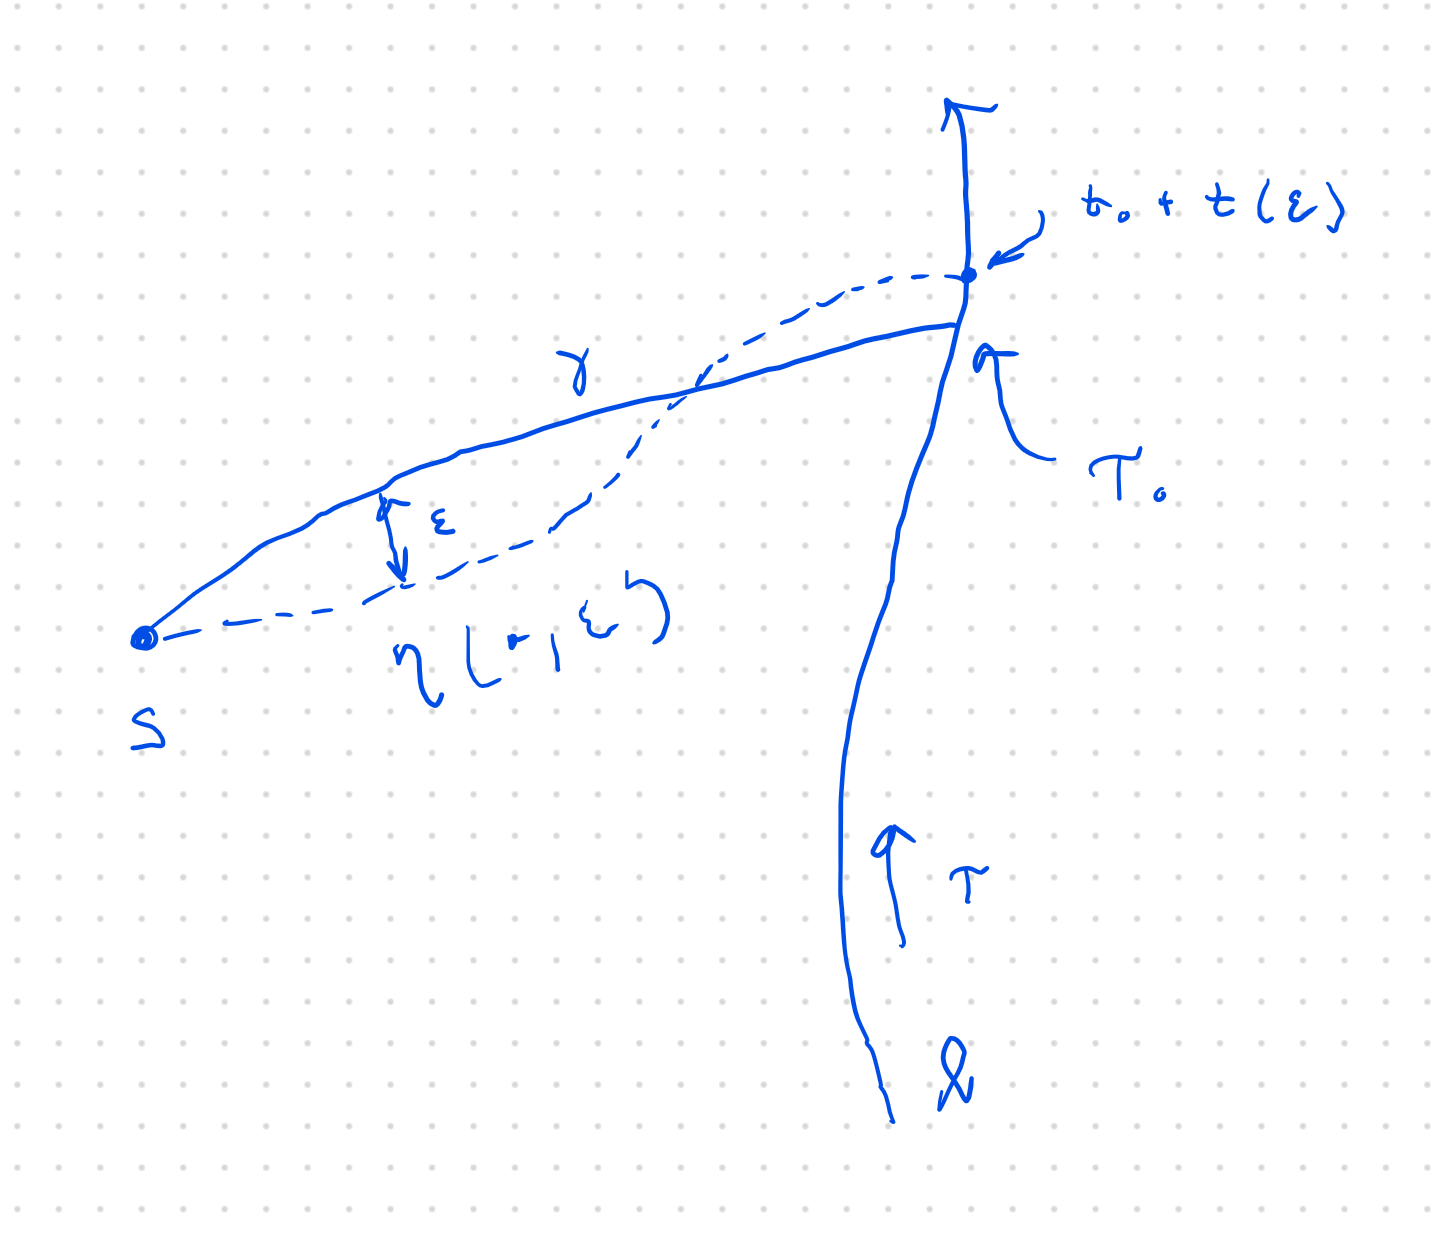
\includegraphics[width=0.5\textwidth]{img/null-variations.png}
	\caption{Family of null variations}
	\label{}
\end{figure}

The action takes the form
\begin{equation}\label{}
S[\gamma_{\eps}] = \int_0^1 L(\eta(\lambda, \eps), \nabla_{\lam} \eta(\lam, \eps)) \, d\lam
\end{equation}
with the Lagrangian
\begin{align*}
L(\eta(\lam, \eps), \veta(\lam, \eps)) &= \frac{1}{2} g (\nabla_{\lam} \eta(\lam, \eps), \nabla_{\lam} \eta(\lam, \eps)) \\
&= \frac{1}{2} g_{\mu, \nu} \rvert_{\gamma(\lam)} \veta^{\mu} (\lam, \eps) \veta^{\nu}(\lam, \eps)
\end{align*}
%
We now differentiate
\begin{align*}
\diff{}{\eps} \frac{1}{2} \int_0^1 g_{\mu \nu} \at_{\gamma(\lam)} \veta^{\mu}(\lam, \eps) \veta^{\nu}(\lam, \eps) \, d\lam
&= \int_0^1 g_{\mu \nu} \at_{\gamma(\lam)} \diff{}{\eps}\brk[s]!{\veta^{\mu}(\lam, \eps)} \veta^{\nu}(\lam, \eps) \, d\lam \\
&= \int_0^1 \veta_{\mu} (\lam, \eps) \diff{}{\eps} \brk[s]!{\veta^{\mu} (\lam, \eps)} \, d\lam
= \int_0^1 \veta_{\mu} (\lam, \eps) \diff{}{\lam} \diff{}{\eps} \eta^{\mu} (\lam, \eps) \, d\lam\\
&= - \int_0^1 \ddot{\eta_{\mu}}(\lam, \eps) \brk[s]!{\diff{}{\eps} \eta^{\mu}(\lam, \eps)} \, d\lam + \brk[s]!{\veta_{\mu} (\lam, \eps) \diff{}{\eps} \brk[r]1{\eta^{\mu}(\lam, \eps)}}^{\lam = 1}_{\lam=0}
\end{align*}
Recall that we have constructed our variation such that $\eta^{\mu}(\lam, \eps) = \xi^{\mu}(\tau_0 + t(\eps))$. Thus the first term simplifies to
\begin{equation}\label{}
-\int_0^1 \ddot{\eta}_{\mu}(\lam, \eps) \dot{\xi}^{\mu}(\tau_0 + t(\eps)) \cdot \dot{t}(\eps) \, d\lam \at_{\eps=0} =
-\int_0^1 \ddot{\gamma}_{\mu}(\lam) \dot{\xi}^{\mu}(\tau_0) \cdot \dot{t}(0) \, d\lam \at_{\eps=0} = 0
\end{equation}
where the last equality is true because $\gamma$ is a geodesic, and therefore must have a affine parameterization (constant speed). The second term yields
\begin{align*}
\brk[s]1{\veta_{\mu} (\lam, \eps) \diff{}{\eps} (\eta^{\mu}(\lam, \eps))}^{\lam = 1}_{\lam = 0}
&= \veta_{\mu} (1, \eps) \diff{}{\eps} (\eta^{\mu}(1, \eps))
-  \veta_{\mu} (0, \eps) \diff{}{\eps} (\eta^{\mu}(0, \eps)) \\
&=\veta_{\mu} (1, \eps) \diff{}{\eps} (\xi^{\mu}(\tau_0 + t(\eps)) \\
&=\veta_{\mu} (1, \eps) \diff{}{\eps} (\dot{\xi}^{\mu}(\tau_0 + t(\eps)) \dot{t}(\eps) \\
&\implies \veta_{\mu} (1, 0) \diff{}{0} (\dot{\xi}^{\mu}(\tau_0 + t(0)) \dot{t}(0)
\end{align*}
Since $\veta$ is lightlike and $\dot{\xi}$ is timelike, their contraction is nonzero. This implies that $\dot{t}(0)$.
%
\\$(\impliedby)$ See \cite{1992grle.book.....S}.
\end{proof}
%
A well known feature of General Relativity is that light rays follow null geodesics in spacetime.
Interestingly, we may show using Fermat's theorem \cite{PerlickV1990OFpi} that null geodesics on a \textbf{stationary} spacetime are in one-to-one correspondence with geodesics on a Finsler-Randers type manifold, and null geodesics on a \textbf{static} spacetime are in one-to-one correspondence with geodesics on a Riemannian manifold. The strategy of optical geometry is to study these simpler spatial geodesics instead. These simpler metrics are called the \textbf{optical metric}, or the \textbf{Fermat metric}.

\begin{definition}[]\label{}
A spacetime $(\man, g)$ is called \textbf{stationary} if there is a timelike killing vector field $T \in \tanb$ satisfying
%
\begin{enumerate}[i)]
  \item $g(T, T) = 0$
  \item $\lie_Tg = 0$
\end{enumerate}
\end{definition}
%
Although this formalism works for stationary spacetimes, we will restrict ourselves to the following special case.
%
\begin{definition}[]\label{}
A spacetime $(\man, g)$ is called \textbf{static} if it is stationary, and its timelike Killing vector field $T$ is \textbf{hypersurface orthogonal}. That is, $T_{[a} \partial_b T_{c]}$.
\end{definition}
It may be shown \cite{straumann2012general} that there exist coordinates for a static spacetime such that the metric decomposes to
\begin{equation}\label{}
g = -V^2 dt^2 + h_{ab} dx^a dx^b
\end{equation}
where $V^2 \defn T^a T_a$, and $h_{ab}$ has $(+, +, +)$ signature.
\begin{remark}[]\label{}
The null geodesics of a Lorentzian metric are unaffected by \textbf{conformal transformations} of the metric. That is, multiplication by positive functions. Since we are interested only in light rays, we may drop the $V^2$ without loss of generality.
\end{remark}
\begin{corollary}[]\label{}
The null geodesics of a static spacetime are equivalent to the geodesics of the purely spatial metric $h=h_{ab} dx^a dx^b$
\end{corollary}
\begin{proof}
Let $\eta$ be a null curve, and consider the proof of Fermat's principle from earlier. Let us consider the special case where the observer is an integral curve of the Killing vector $T$, such that
\begin{equation}\label{}
l^{\mu} = (\lambda, x_1, x_2, x_3)
\end{equation}
The fact that $\eta$ must be a null curve provides a relationship between its derivative components
\begin{equation}\label{}
\dot{\eta}^0 = \sqrt{h_{ij} \dot{\eta}^i \dot{\eta}^j}
\end{equation}
We know that $\eta^0(0) = const$, $\eta^0(1) = \tau(\eta)$. Therefore
\begin{align*}
\int_0^1 \dot{\eta}^0 &= \dot{\eta}^0(1) - \dot{\eta}^0(0) = \int_0^1 \sqrt{h_{ij} \dot{\eta}^i \dot{\eta}^j} \\
&\implies \tau(\eta) = \int_0^1 \sqrt{h_{ij} \dot{\eta}^i \dot{\eta}^j} ds + const
\end{align*}
Note that since static metrics have time independent components, the RHS is independent of time, and resembles the length functional on a Riemannian manifold with metric $h$. By Fermat's theorem, varying this length functional will return a null geodesic of the original spacetime.
\end{proof}

%
% Using this definition we may obtain constraints on what a stationary metric must look like in coordinates. First, we have the following result.
% \begin{corollary}[]\label{}
% Suppose $(\man, g)$ is a stationary spacetime. Then there exists a chart for which components of the metric are time independent.
% \end{corollary}
% \begin{proof}
% Suppose we pick a chart such that the vector field $T$ may be expressed as $T = \delta^{\mu}_0 \diffp{}{x^{\mu}}$. Thus
% \begin{align*}
% (\lie_T g)_{\mu \nu} &= T^{\lam} g_{\mu \nu, \lam} + g_{\lam \nu} T^{\lam}_{,\mu} + g_{\mu \lam} T^{\lam}_{,\nu} = g_{\mu \nu, 0} = 0
% \end{align*}
% \end{proof}
%
% We may now write down the most general spacetime satisfying this property
% %
% \begin{equation}\label{}
% g = g_{\mu \nu} dx^{\mu} \otimes dx^{\nu} = -V^2(dt + \omega_a dx^a)^{\otimes 2} + h_{ab} dx^a \otimes dx^b
% \end{equation}
% %
% where $V$ is a positive function representing the norm of the Killing field, $h_{ab}$ form the components of a Riemann metric, and $\omega_a$ is the 3-vector called the \textbf{twist vector}, which measures the extent to which $T$ fails to be orthogonal to a family of three surfaces. Such a metric is known as a \textbf{Finsler-Randers} metric.
% In matrix form, the components of the metric take the form:
% $$
% [g_{\mu \nu}] =
% \begin{pNiceArray}{C|C}
% -V^2 & -v^2 \omega^{\top} \\
% \hline
% -V^2 \omega & h \\
% \end{pNiceArray}
% $$
% \begin{definition}[]\label{}
% A spacetime $(\man, g)$ is called \textbf{static} if it is stationary, and the twisting vector is zero.
% \end{definition}

\section{Optical geometry of Schwarzschild}
In this section, we will discuss as a particular example the optical geometry of the Schwarzschild metric. Recall that the Schwarzschild metric is given by
\begin{equation}\label{}
ds^2 = -\brk[r]2{1-\frac{2m}{r}} dt^2 + \frac{dr^2}{1-\frac{2m}{r}} + r^2(d\theta^2 + sin^2\theta d\phi^2)
\end{equation}
Without loss of generality we only consider the equatorial plane $\theta=\frac{\pi}{2}$. To build intuition for this geometry we aim to find an isometric embedding into three dimensional Euclidean space $\mathbb{E}^3$. We proceed in cylindrical coordinates, and solve for the null geodesics
% \begin{equation}\label{}
% dt^2 = \frac{dr^2}{\brk[r]1{1 - \frac{2m}{r}}^2} + \frac{r^2}{1 - \frac{2m}{r}} d\phi^2
% \end{equation}

\begin{align*}
dt^2 &= \frac{dr^2}{\brk[r]1{1 - \frac{2m}{r}}^2} + \frac{r^2}{1 - \frac{2m}{r}} d\phi^2 = dz^2 + dR^2 + R^2 d\phi^2
\end{align*}
The following result will help us visualize this surface.
\begin{proposition}[]\label{}
Let $(z, R, \phi)$ denote cylindrical coordinates. Then for the equatorial plane of the Fermat-Schwarzschild metric the following holds:
\begin{equation}\label{}
\brk[r]2{\diff{z}{R}}^2 = \frac{4mr-9m^2}{(r-3m)^2}
\end{equation}
\end{proposition}
\begin{proof}
The following will be used to simplify the algebra
\begin{align*}
f(r) &\defn \sqrt{1 - \frac{2m}{r}} \\
f'(r) &= \frac{1}{2}\brk[r]2{1-\frac{2m}{r}}^{-\frac{1}{2}}\frac{2m}{r^2} = \frac{m}{r^2f} \\
f^4 &= \brk[r]2{1 - \frac{2m}{r}}^2 = 1 + \frac{4m^2}{r^2} - \frac{4m}{r}
\end{align*}
Observe that $R(r) = \frac{r}{f}$. Likewise,
\begin{equation}\label{}
\diff{R}{r} = \diff{}{r} \brk[r]2{\frac{r}{f}} = \frac{f - rf'}{f^2} = f^{-1} - \frac{m}{rf^3} = \frac{rf^2 - m}{rf^3}
\end{equation}
We find an expression for $\diff{z}{R}$.
\begin{align*}
\frac{1}{f^4} + \frac{r^2}{f^2} \brk[r]2{\diff{\phi}{r}} &= \brk[r]2{\diff{z}{r}} + \brk[r]2{\diff{R}{r}} + R^2 \brk[r]2{\diff{\phi}{r}} \\
\implies \frac{1}{f^4} &= \brk[r]2{\diff{z}{r}}^2 + \brk[r]2{\diff{R}{r}}^2 = \brk[r]2{\diff{z}{R}}^2 \brk[r]2{\diff{R}{r}}^2 + \brk[r]2{\diff{R}{r}}^2 = \brk[s]2{\brk[r]2{\diff{z}{R}}^2 + 1}\brk[r]2{\diff{R}{r}}^2 \\
\implies \brk[r]2{\diff{z}{R}}^2 &= \frac{1}{f^4} \brk[r]2{\diff{R}{r}}^{-2} - 1 = \frac{r^2 f^6}{(rf^2 + m)^2} - 1 \\
\implies (rf^2-m)^2 &= r^2f^4 - 2rf^2m + m^2 \\
&= r^2 \brk[r]2{1 - \frac{2m}{r}^2} - 2r \brk[r]2{1 - \frac{2m}{r}}m + m^2 \\
&= r^2 \brk[r]2{1 - \frac{4m}{r} + \frac{4m^2}{r^2}} - 2rm + 4m^2 + m^2 \\
&= r^2 - 4mr + 4m^2 - 2rm + 4m^2 + m^2 \\
&= r^2 - 6mr + 9m^2 \\
\implies \brk[r]2{\diff{z}{R}}^2 &= \frac{r^2 \brk[r]2{1 - \frac{2m}{r}}}{r^2 - 6mr + 9m^2} + \frac{-r^2 + 6mr - 9m^2}{r^2 - 6mr + 9m^2} \\
&= \frac{4mr - 9m^2}{(r-3m)^2}
\end{align*}
as expected.
\end{proof}
In light of the previous calculation, we make the following observations:
\begin{enumerate}[i)]
\item The embedding is restricted to $4mr - 9m^2 > 0 \implies 4r > 9m \implies r > \frac{9}{4}m$ and therefore does not work for $2m < r < \frac{9}{4}m$.
\item Observe that asymptotically, $R \rightarrow r$. Hence
\begin{equation}\label{}
\lim_{r \uparrow \infty} \brk[r]2{\diff{z}{R}}^2 = \frac{4mR}{R^2} = \frac{4m}{R} \implies \diff{z}{R} = 2\sqrt{\frac{m}{R}}
\end{equation}
I.e, $z$ goes as $\sqrt{R}$ asymptotically
\item
$\diff{z}{R}$ is singular at $R(r=3m)$. This corresponds to the circular photon orbit of Schwarzschild.
\end{enumerate}
%
A surface with these properties is represented in \ref{fig:embedding}.
Visually, it appears as though this surface has everywhere negative Gaussian curvature. Indeed this is case, and may be shown analytically.
\begin{proposition}[]\label{}
The Gaussian curvature associated with the Fermat metric of equatorial Schwarzschild has everywhere negative curvature. Specifically, for $r > 2m$,
\begin{equation}\label{}
K = - \frac{2m}{r^3}\brk[r]2{1 - \frac{3m}{2r}}
\end{equation}
\end{proposition}
%
\begin{figure}[!htb]
	\centering
	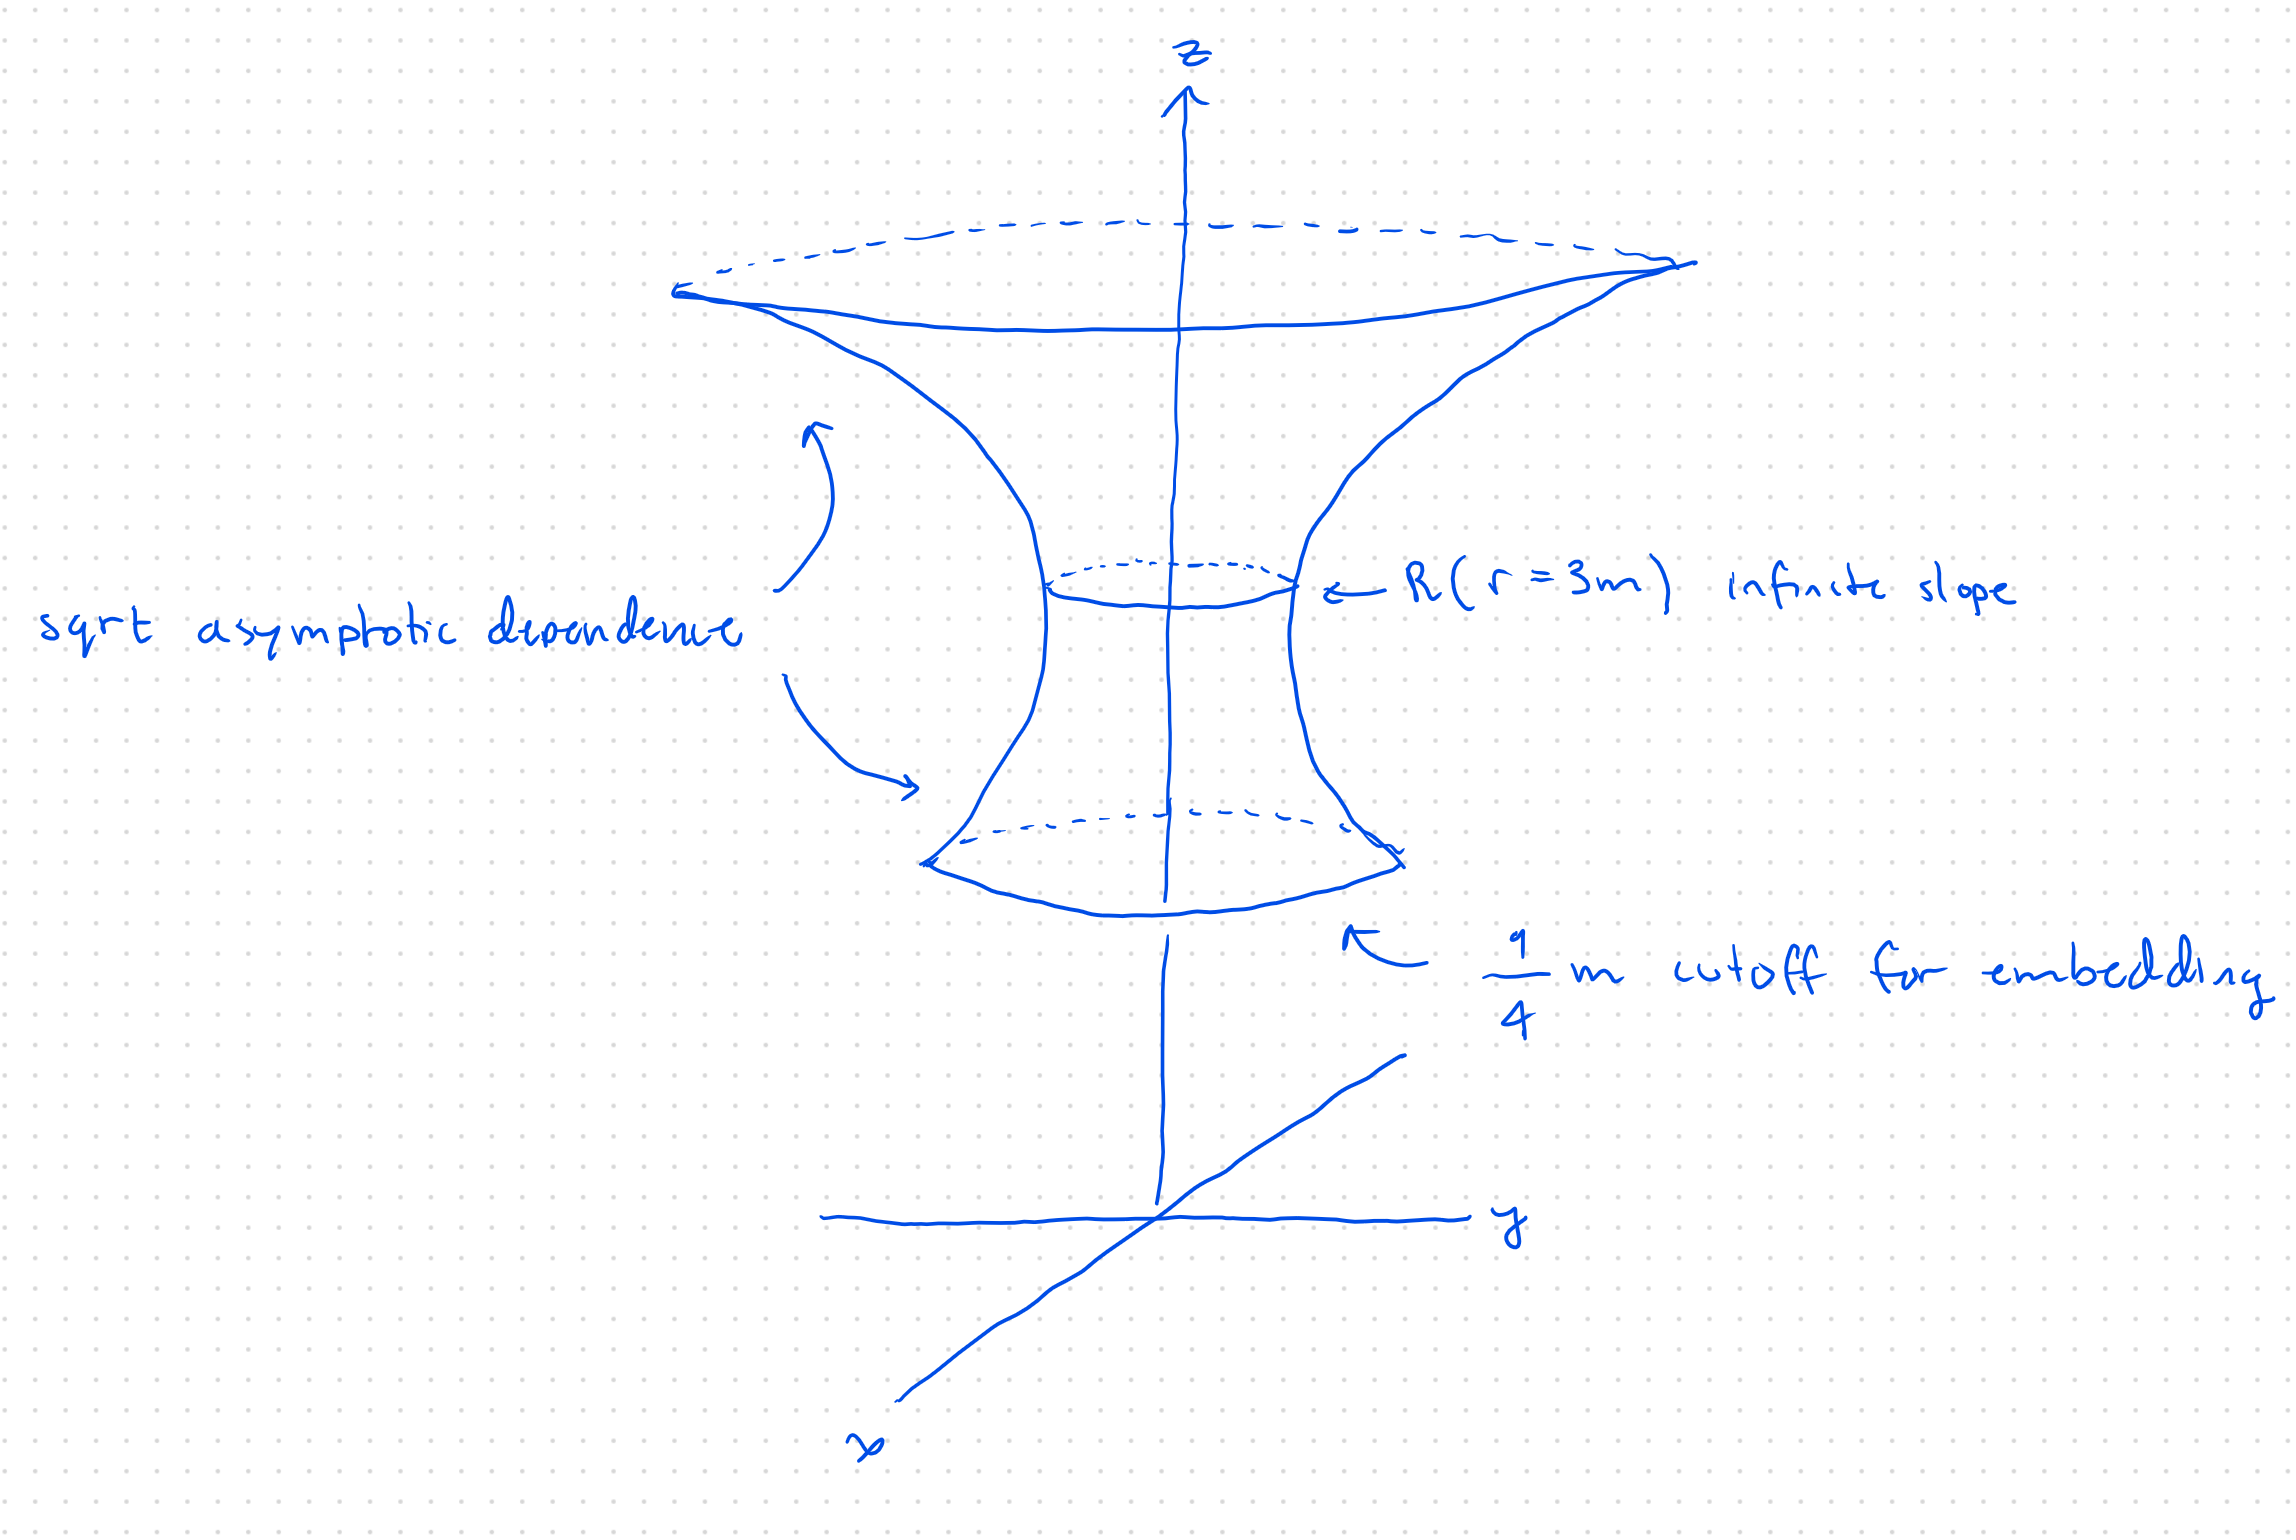
\includegraphics[width=0.95\textwidth]{img/embedding.png}
	\caption{The embedding in $\mathbb{E}$ of the equatorial Schwarzschild-Fermat metric.}
	\label{fig:embedding}
\end{figure}

\section{Gauss-Bonnet and gravitational lensing}
We are now in possession on a negatively curved surface $\Sigma$ on which geodesic behavior tells us about the behavior of light rays on the equatorial plane of Schwarzschild. We may now use well known results from surface analysis to tease out the physics we are interested in.
\begin{question}[]\label{}
Under what circumstances can two geodesics with the same initial point $s \in \Sigma$ (source) meet at another point $o \in \Sigma$ (observer)?
\end{question}
The answer to this condition will tell us under what conditions one may observe multiple images! An interesting result is that negative curvature causes geodesics on the surface to diverge on small scales. Indeed, the following result is a precise statement.
\begin{theorem}[]\label{}
Let $\gamma: I \to \Sigma$ be a curve in $\Sigma$ such that $\gamma(0)=p$, $\dot{gamma}(0) = v$. Now, let $J$ be a Jacobi field along $\gamma$ satisfying $J(0)=0$, $J'(0)=w$, and suppose $g(v,v)=g(w,w)=1$. Then
\begin{equation}\label{}
\norm{J(t)} = t - \frac{K}{6}t^3 + \order(t^4)
\end{equation}
where $K$ is the Gaussian curvature of $Sigma$.
\end{theorem}




\begin{theorem}[]\label{}
Suppose $M$ is a compact two dimensional Riemannian manifold with boundary. Let $K$ be the Gaussian curvature of M, and let $k_g$ be the geodesic curvature on the boundary. Then
\begin{equation}\label{}
\int_M K \, dA + \int_{\partial M} k_g \, ds = 2 \pi \xi(M)
\end{equation}
where $dA$ is area element, $ds$ is the line element along the boundary, and $\xi(M)$ is the Euler characteristic of $M$.
\end{theorem}
